%!TeX root= ../thesis.tex
\section{UML}


\begin{center}
	\begin{tikzpicture}
		\umlclass[y=-3]{Class}{
			d : double
		}{ equals(c : Class) : boolean \\ toString() : String \\ hashCode() : Integer}
	\end{tikzpicture}
\end{center}

\begin{sidewaysfigure}[h]
	\centering
	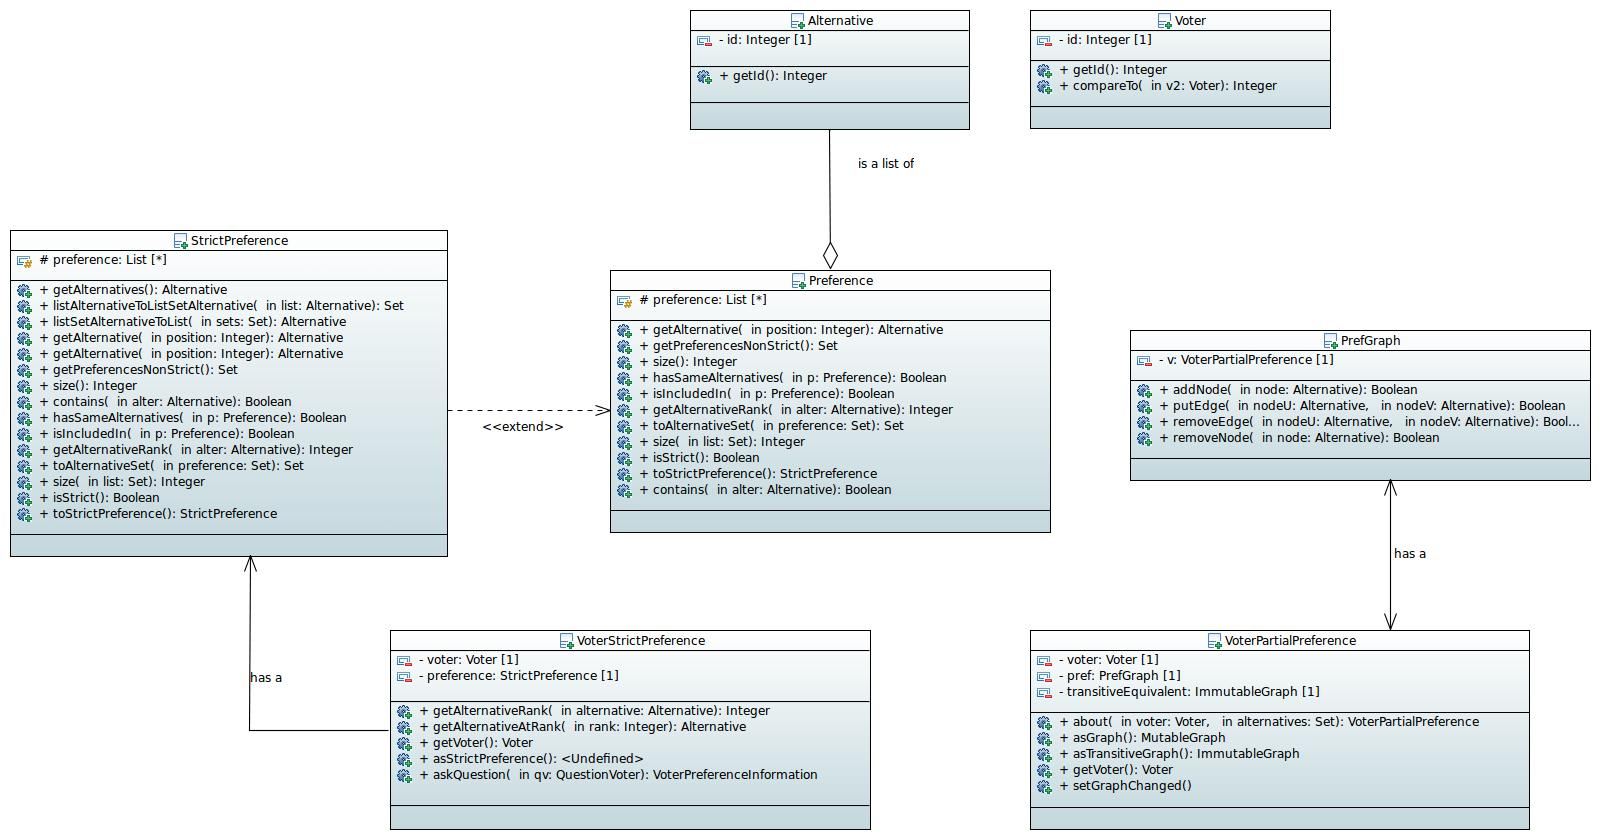
\includegraphics[width=\textwidth]{uml/Basic.jpeg}
	\caption{UML class diagram of preferences representation.}
\end{sidewaysfigure}

\begin{sidewaysfigure}[h]
	\centering
	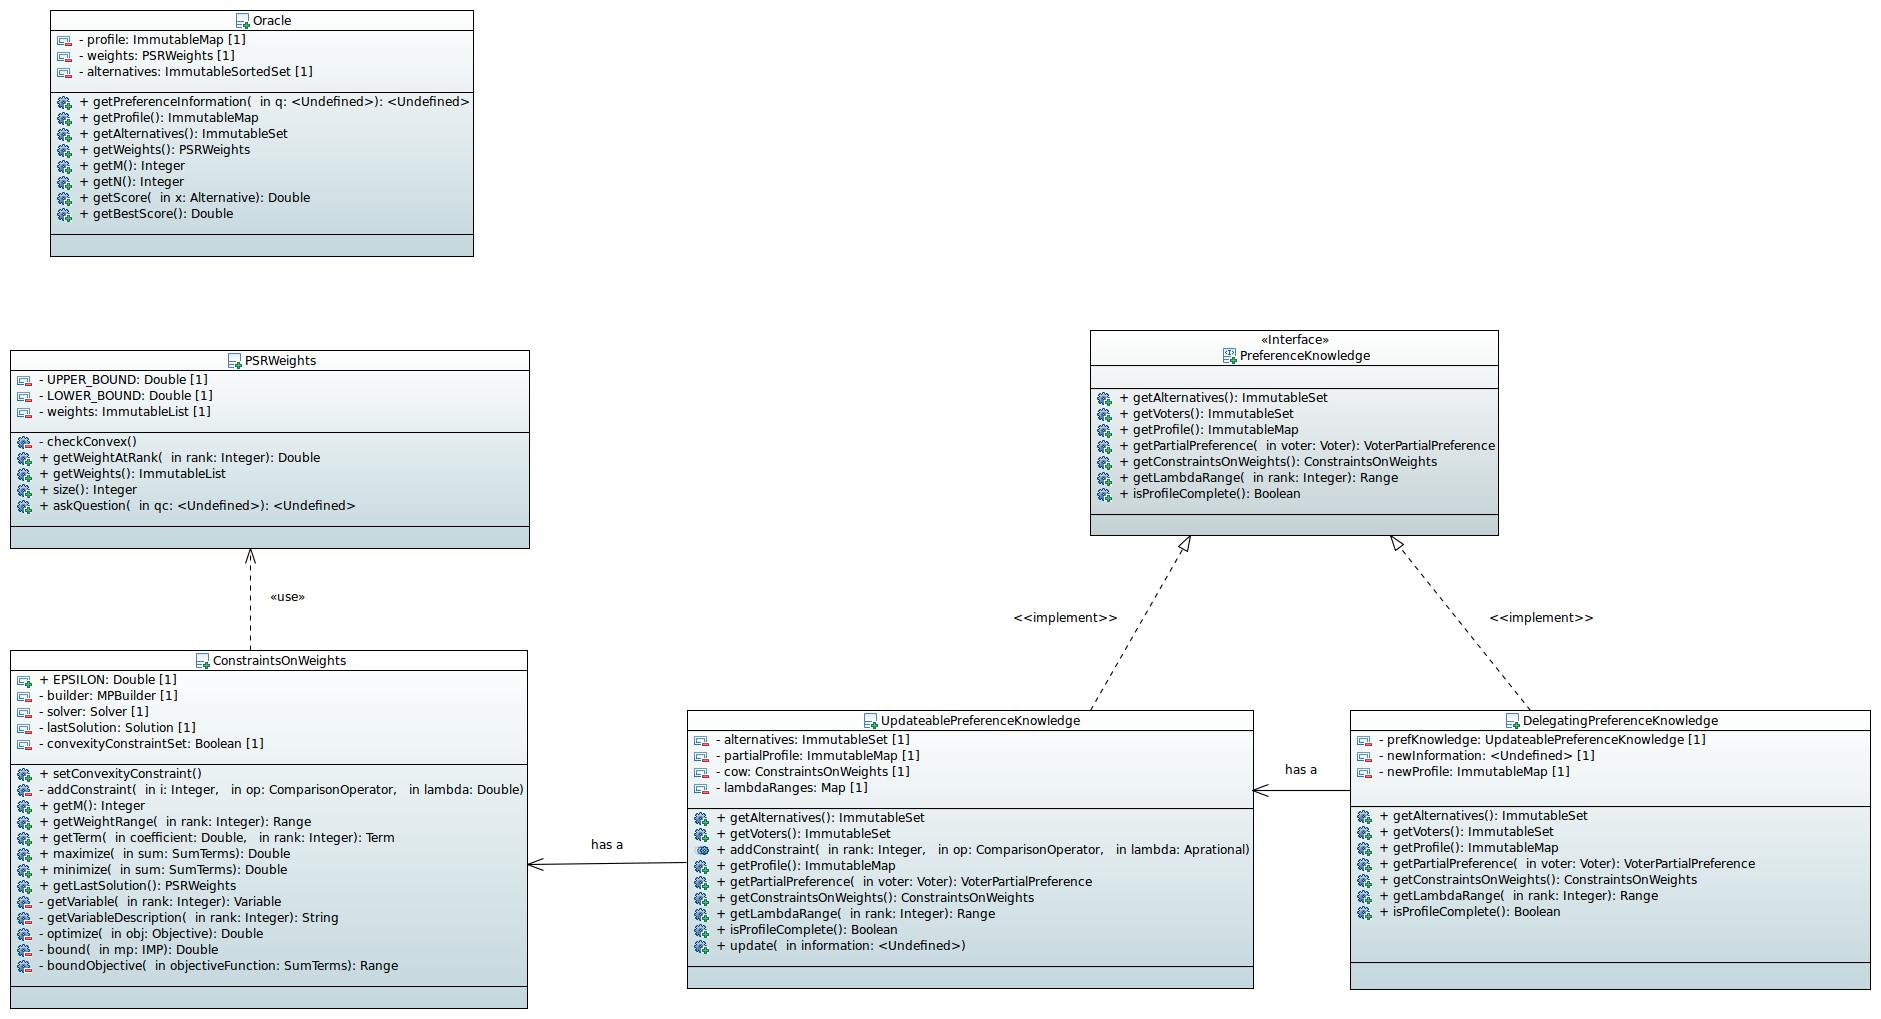
\includegraphics[width=\textwidth]{uml/model.jpeg}
	\caption{UML class diagram of knowledge representation.}
\end{sidewaysfigure}

\begin{figure}[h]
	\centering
	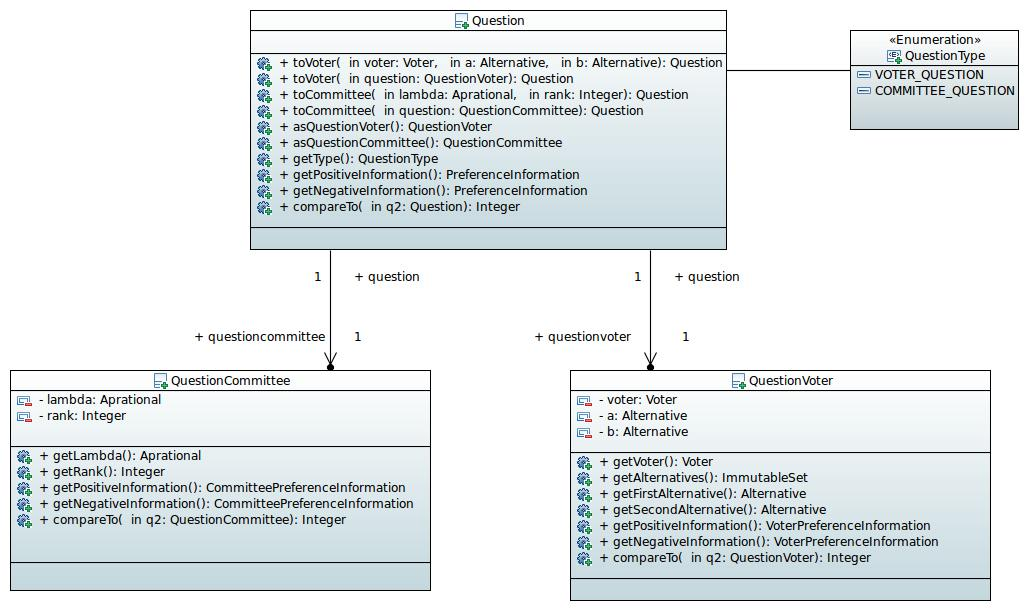
\includegraphics[width=\textwidth]{uml/questions.jpeg}
	\caption{UML class diagram of questions representation.}
\end{figure}

\begin{figure}[h]
	\centering
	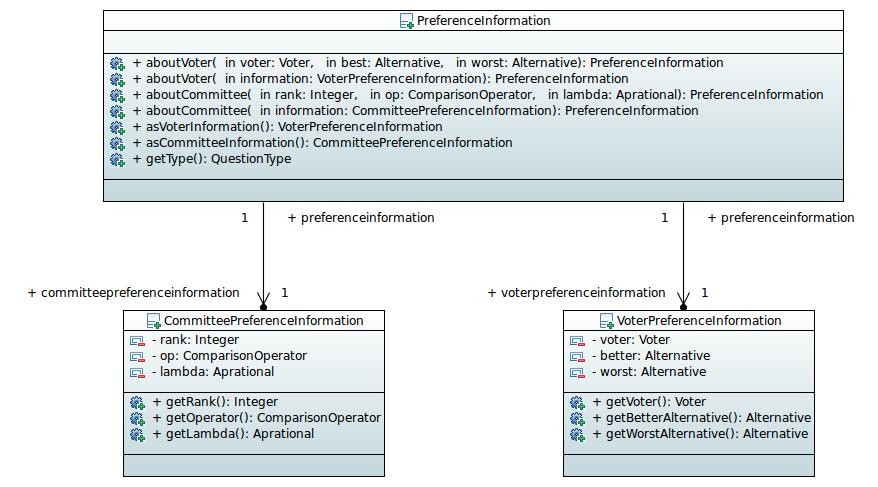
\includegraphics[width=\textwidth]{uml/prefinfo.jpeg}
	\caption{UML class diagram of elicited knowledge obtained by asking questions.}
\end{figure}

\begin{figure}[h]
	\centering
	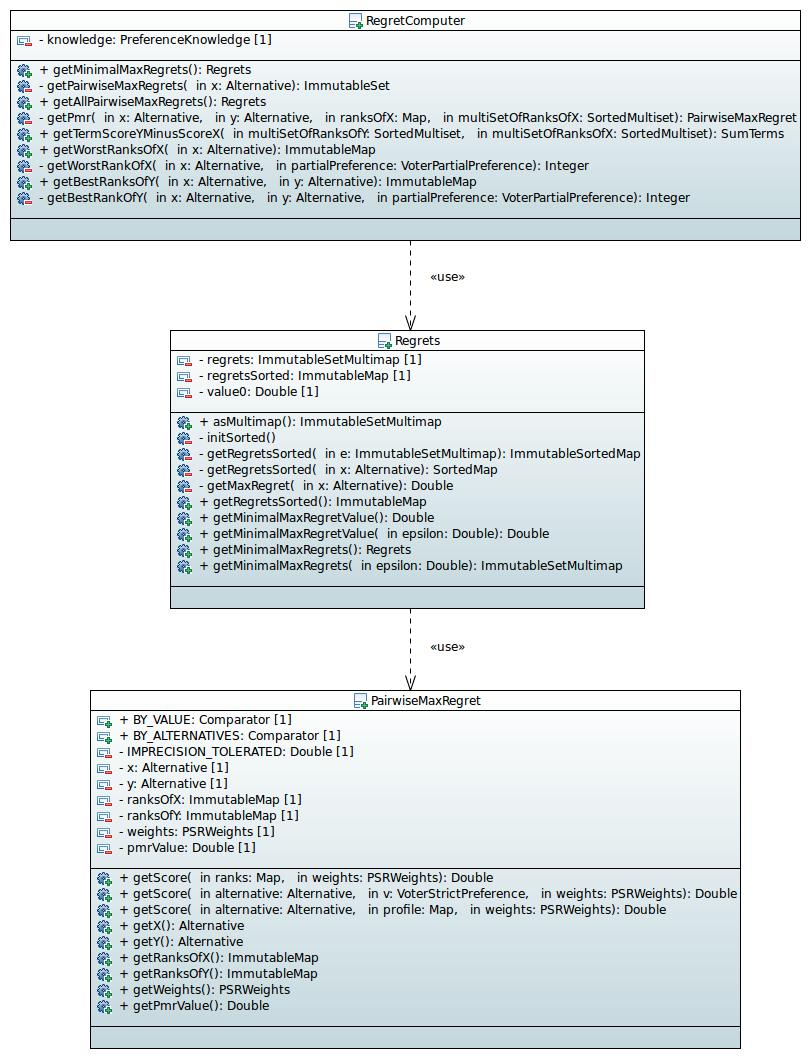
\includegraphics[width=\textwidth]{uml/regret.jpeg}
	\caption{UML class diagram of regret computation.}
\end{figure}

\begin{sidewaysfigure}[h]
	\centering
	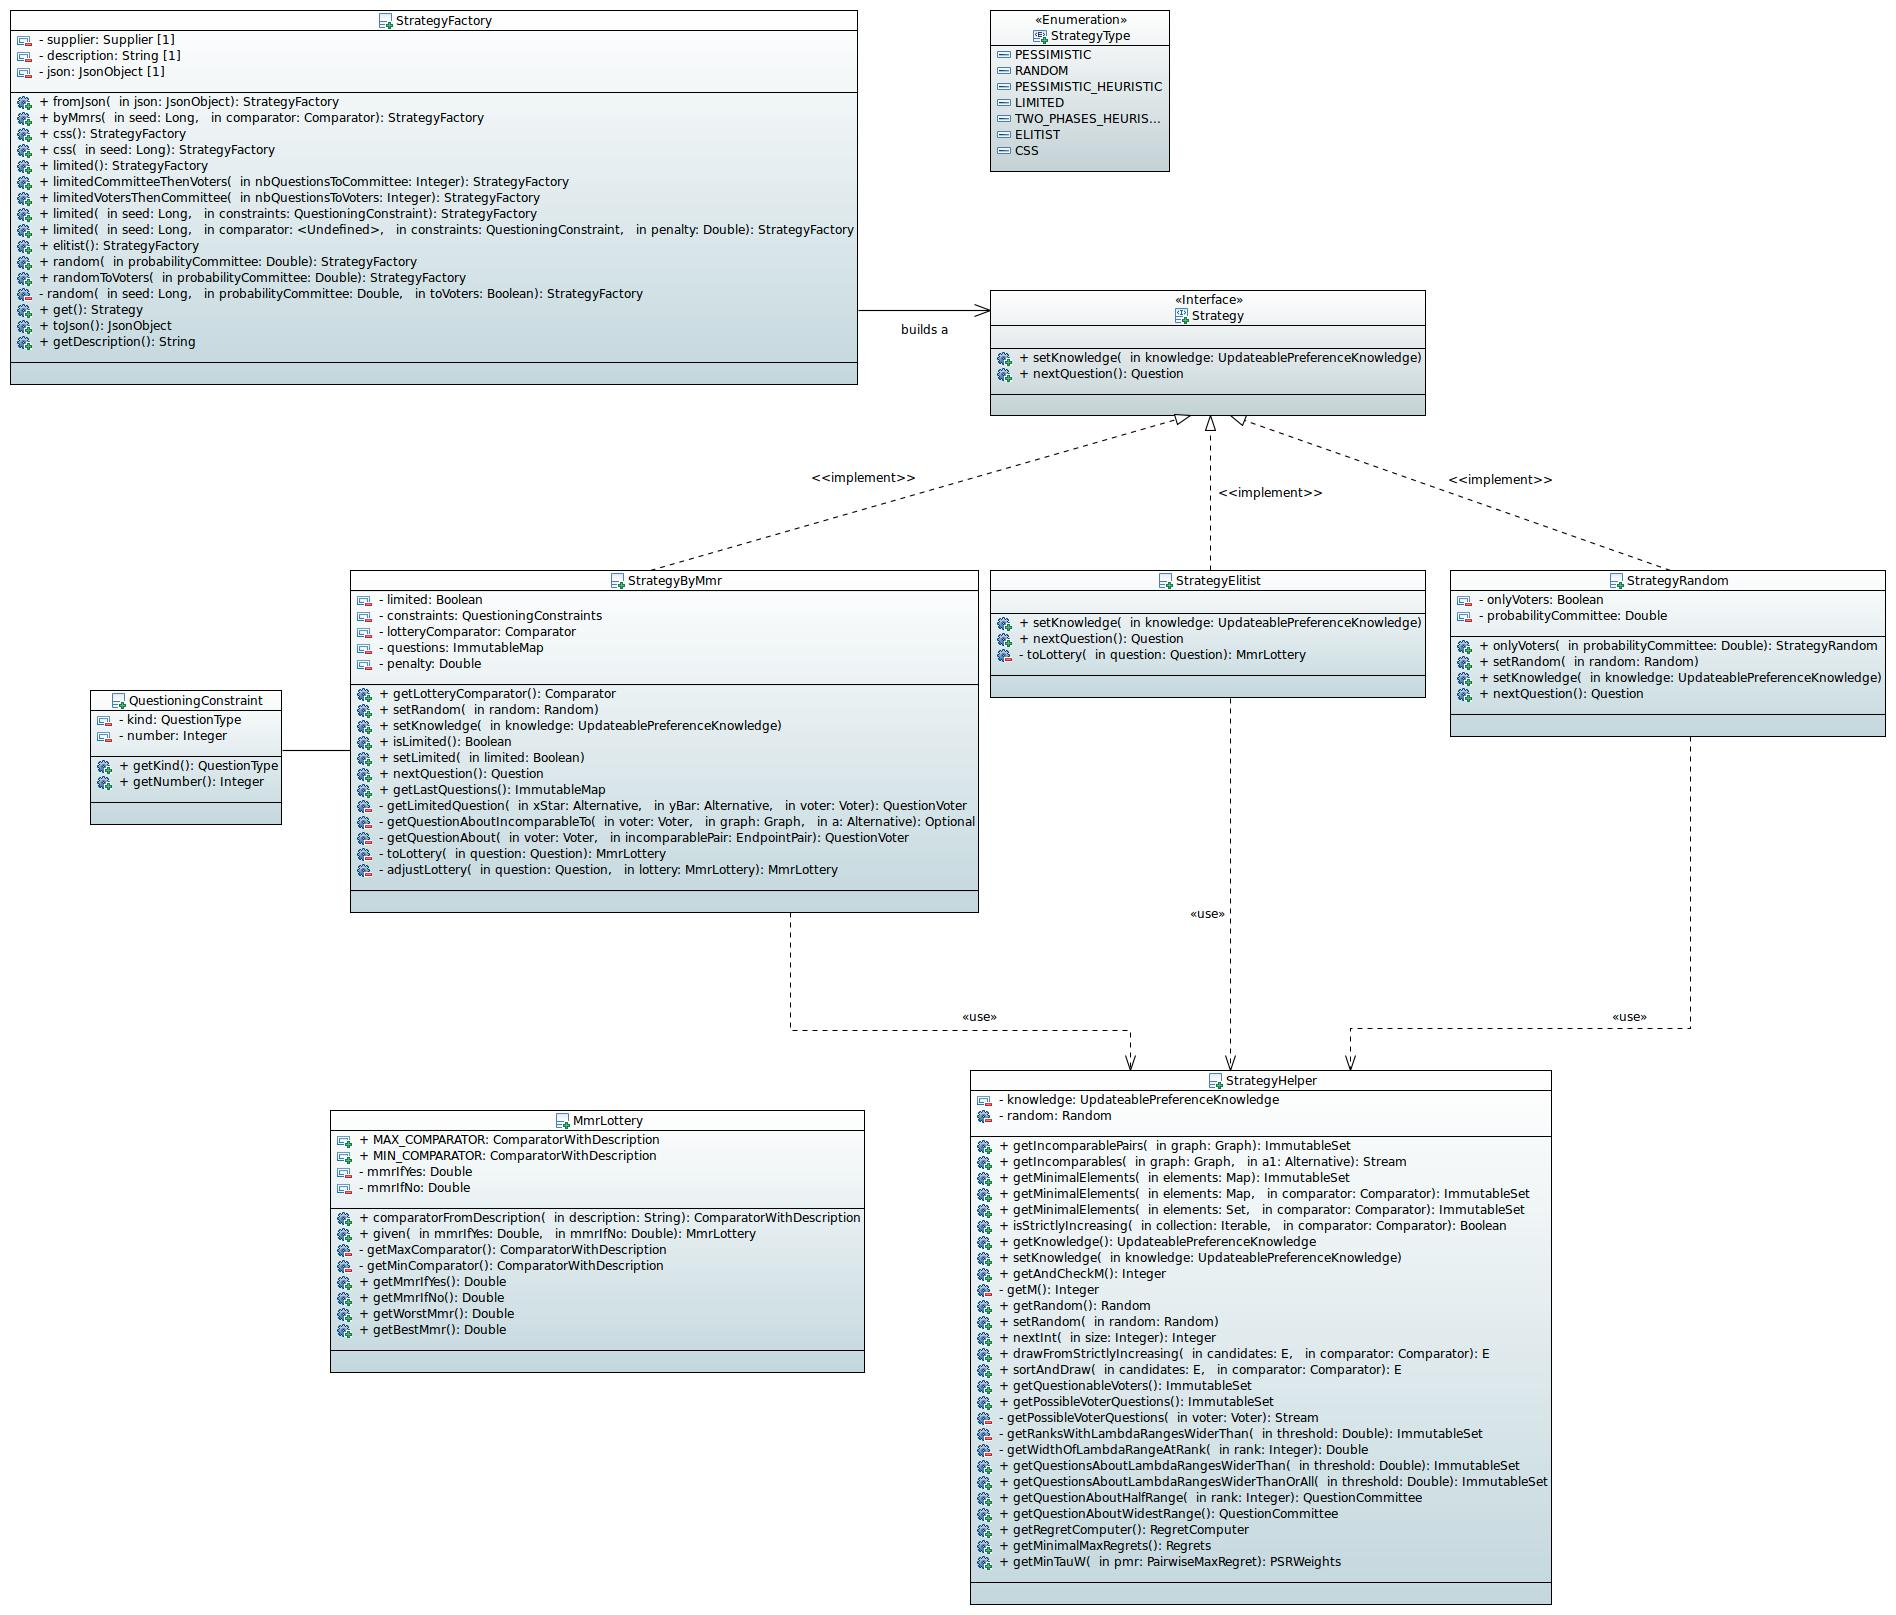
\includegraphics[width=\textwidth]{uml/strategies.jpeg}
	\caption{UML class diagram of strategies.}
\end{sidewaysfigure}

%\begin{center}
	%	\begin{tikzpicture}
	%		\begin{umlpackage}{p}
	%			\begin{umlpackage}{sp1}
	%				\umlclass[template=T]{A}{
	%					n : uint \\ t : float
	%				}{}
	%				\umlclass[y=-3]{B}{
	%					d : double
	%				}{
	%					\umlvirt{setB(b : B) : void} \\ getB() : B}
	%			\end{umlpackage}
	%			\begin{umlpackage}[x=10,y=-6]{sp2}
	%				\umlinterface{C}{
	%					n : uint \\ s : string
	%				}{}
	%			\end{umlpackage}
	%			\umlclass[x=2,y=-10]{D}{
	%				n : uint
	%			}{}
	%		\end{umlpackage}
	%		
	%		\umlassoc[geometry=-|-, arg1=tata, mult1=*, pos1=0.3, arg2=toto, mult2=1, pos2=2.9, align2=left]{C}{B}
	%		\umlunicompo[geometry=-|, arg=titi, mult=*, pos=1.7, stereo=vector]{D}{C}
	%		\umlimport[geometry=|-, anchors=90 and 50, name=import]{sp2}{sp1}
	%		\umlaggreg[arg=tutu, mult=1, pos=0.8, angle1=30, angle2=60, loopsize=2cm]{D}{D}
	%		\umlinherit[geometry=-|]{D}{B}
	%		\umlnote[x=2.5,y=-6, width=3cm]{B}{Je suis une note qui concerne la classe B}
	%		\umlnote[x=7.5,y=-2]{import-2}{Je suis une note qui concerne la relation d'import}
	%	\end{tikzpicture}
%\end{center}